% -*- coding: utf-8; mode: latex; -*-

% jlreq.cls を使う、二段組、和文フォントスケールは pTeX のデフォルト相当
\documentclass[twocolumn,jafontscale=0.962216,jlreq_notes]{jlreq}

% LuaTeX-ja を使う
\usepackage{luatexja}
% 和文フォントは源ノ明朝 / 源ノ角ゴシックを使う、
% 複数のウェイトを使う、欧文フォントのファミリ指定と連動させる
\usepackage[sourcehan,deluxe,match]{luatexja-preset}

% 最終ページの各段の行数を揃える
\usepackage{nidanfloat}
\usepackage[keeplastbox]{flushend}

\usepackage{graphicx}  % 図の貼り込み用
\usepackage{fancyhdr}  % 表紙右上にヘッダを出すため
\usepackage{hyperref}  % しおり、リンク生成用
\usepackage{hologo}    % 各種 TeX ロゴ用
\usepackage{listings}  % ソースファイル表示用
\usepackage{tcolorbox} % 枠囲み用

% 数式フォント、欧文フォント設定
\usepackage{unicode-math}
\unimathsetup{math-style=ISO,bold-style=ISO}
\setmainfont{Libertinus Serif}
\setsansfont{Libertinus Sans}
\setmonofont{Source Code Pro}[Scale=MatchLowercase] %これだけ大きく見えるので
\setmathfont{Libertinus Math}

% \section などの見出しをゴシック太字からゴシックへ変更
\makeatletter
\ModifyHeading{section}{font={\jlreq@keepbaselineskip{\Large\sffamily}}}
\ModifyHeading{subsection}{font={\jlreq@keepbaselineskip{\large\sffamily}}}
\ModifyHeading{subsubsection}%
              {font={\jlreq@keepbaselineskip{\normalsize\sffamily}}}
\makeatother

% abstract 環境の見出しをゴシック太字からゴシックへ変更
\edef\abstractnamebackup{\abstractname}
\renewcommand{\abstractname}{\mdseries{\abstractnamebackup}}

% caption 関係のフォントをゴシック太字からゴシックへ変更
\jlreqsetup{caption_font={\sffamily},caption_label_font={\sffamily}}

% 表紙のヘッダ指定
\lhead{}
\chead{}
\rhead{%
  \smash{\vtop{%
    TeXConf 2017(2017年10月14日) \\
    Copyright (C) 2017 Masamichi Hosoda \\
    \href{https://creativecommons.org/licenses/by-sa/4.0/deed.ja}%
         {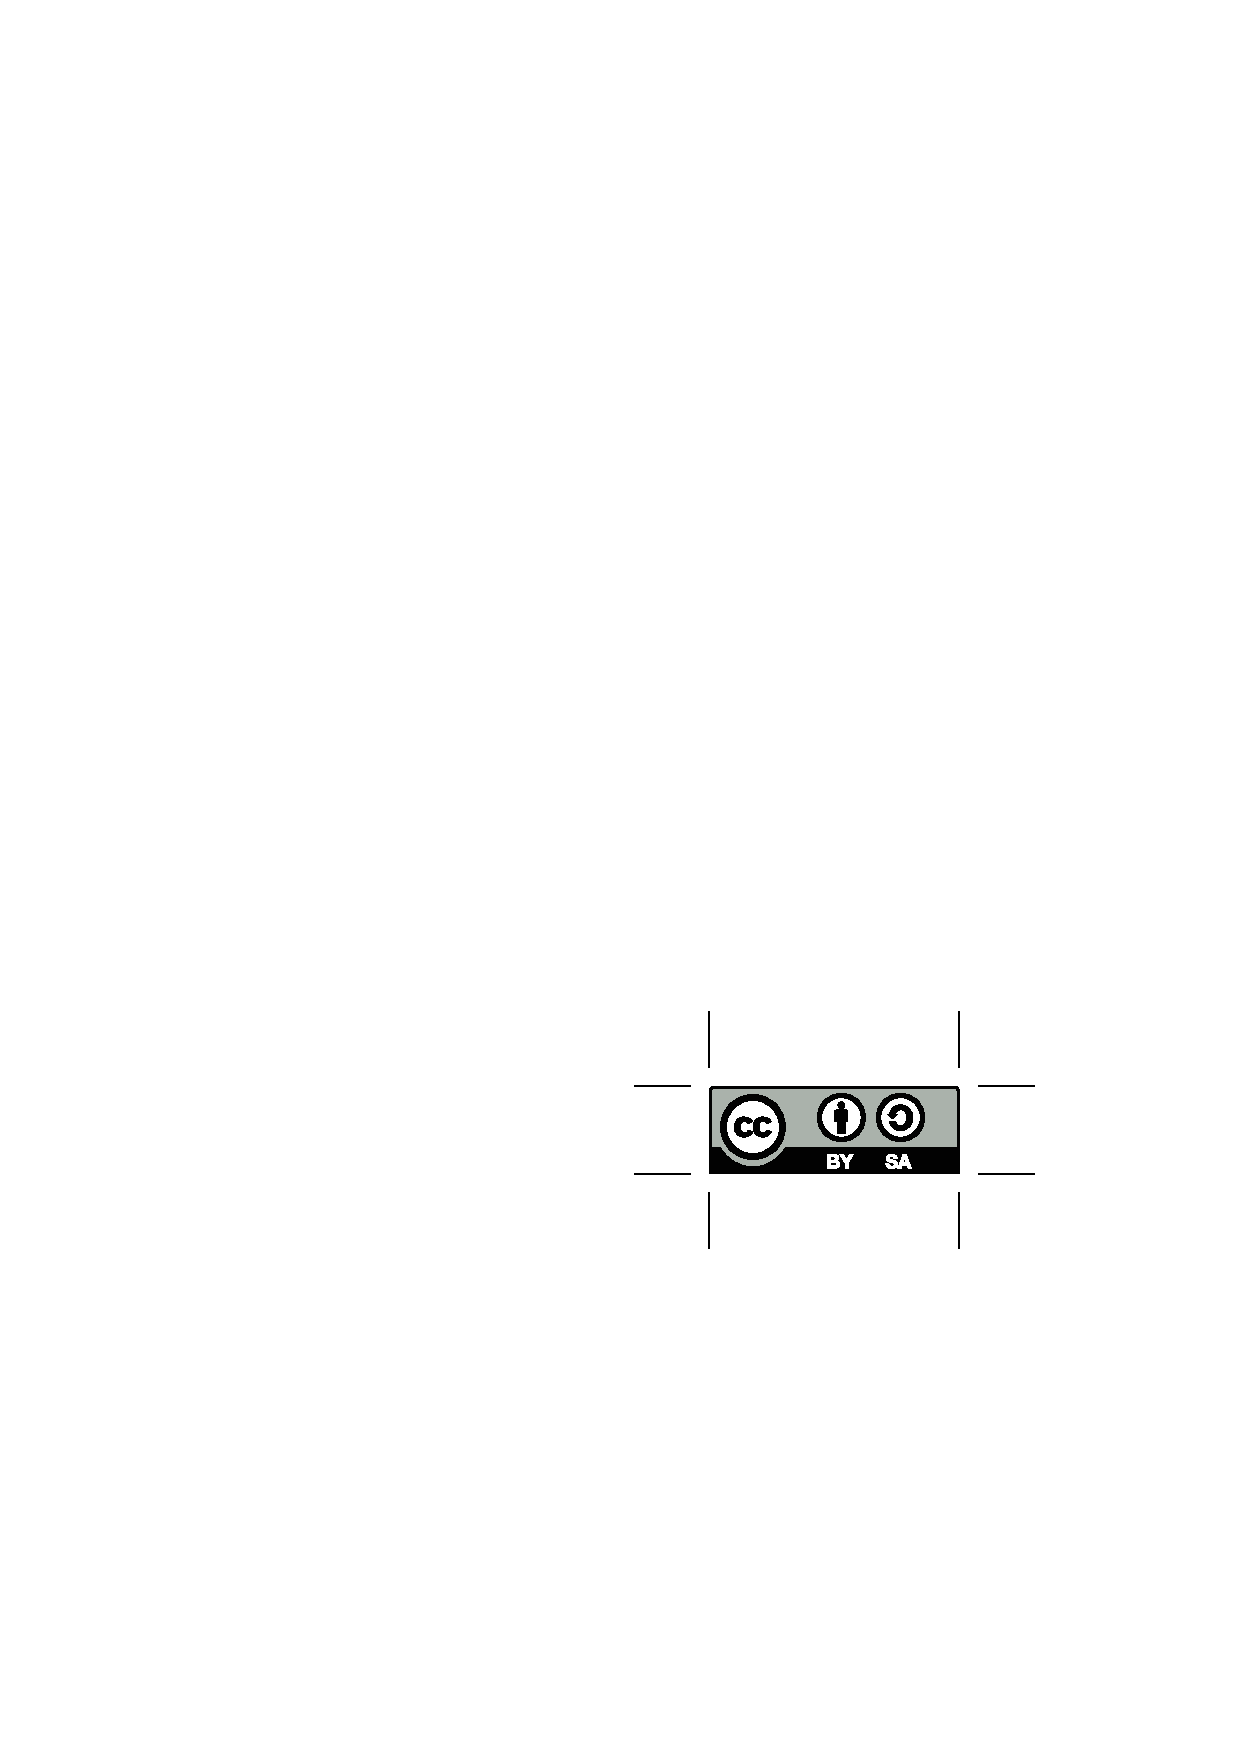
\includegraphics[height=3ex]{by-sa}}}}}
\lfoot{}
\cfoot{\thepage}
\rfoot{}
\renewcommand{\headrulewidth}{0pt}

% hyperref 設定
\hypersetup{%
  unicode=true,% LuaLaTeX 利用のため
  bookmarks=true,% しおり生成
  bookmarksnumbered=true,% しおりに節番号などを付与
  colorlinks=true,% リンクをカラー表示(非ボックス表示)
  urlcolor=blue,% \url リンク色指定
  citecolor=black,% \cite リンク色指定
  linkcolor=black,% \ref リンク色指定
  pdftitle={Extract PDFmarkによるPDFファイルサイズ削減},% タイトル
  pdfsubject=={TeXConf 2017},% サブタイトル
  pdfauthor={細田 真道},% 著者
  pdfkeywords={% キーワード
    Extract PDFmark, extractpdfmark, LilyPond, Texinfo, TeX, LaTeX,
    Ghostscript, PDF%
  },%
}
% \url で表示するURLのフォントを等幅フォントからローマン体へ変更
\renewcommand\UrlFont{\rmfamily}

% listings 設定
\lstset{%
  basicstyle=\small\ttfamily,% フォント設定
  frame=none,% 枠を付けない(listings の枠線は隙間が空いてしまうので)
  lineskip=-0.6ex% 行間を詰める
}

\title{\textsf{Extract PDFmarkによるPDFファイルサイズ削減}}
\author{細田 真道 \\ \url{http://www.trueroad.jp}}
\date{} % 日付表示を抑制

\begin{abstract}
\TeX などで同じフォントが埋め込まれた多数の図PDFを貼り込むと、
結果として生成されるPDFには同じフォントが重複して埋め込まれ、
ファイルサイズ増加につながる。
Ghostscriptで処理することにより埋め込み制御もできるが、
PDFの開き方やリモートからのリンクが失われる。
本稿ではExtract PDFmarkによって、
これらを失わずにファイルサイズの小さいPDFを得る方法を説明する。
\end{abstract}

\begin{document}

\maketitle
\thispagestyle{fancy}

\section{はじめに}

各種の\TeX や\LaTeX などを使ってPDFのドキュメントを作る場合、
図としてたくさんの小さなPDFを用意して、
メインのPDFに貼り付けるようなことが行われる。
このとき、図のPDFでは同じフォントを使っていることが多いと思われる。

楽譜作成プログラムLilyPond \cite{lilypond}のマニュアルは
GNU公式文書フォーマットであるTexinfo \cite{texinfo}形式の
ソースファイルを\hologo{XeTeX}で処理し、PDFを生成している。
楽譜作成プログラムという性格上マニュアルには楽譜の断片を多数含み、
これらはLilyPondでPDFとして生成したものを図として貼り込んでいる。
もちろん、各々の楽譜の断片には同じフォントが使われていることが多い。

一般的に、図PDFにフォントが埋め込まれていた場合、
そのフォントはそのままメインPDFに埋め込まれる。
同じフォントが埋め込まれている複数の図PDFを貼り込むと、
メインPDFにはフォントが重複して複数回埋め込まれることになり
ファイルサイズの増加につながる。

図PDF作成時にフォントの埋め込み方法を工夫し、
メインPDFをGhostscript処理により埋め込み制御をして
ファイルサイズを削減することもできる。
しかし残念ながら、この処理でGhostscriptはPDFのページモードや
リンクの宛先名を残さないため、
処理後のPDFは意図したとおりに開かれなくなったり、
リモートからのリンクが機能しなくなったりする。

本稿では、この問題を解決する方法
としてExtract PDFmark \cite{extractpdfmark}を紹介する。
Extract PDFmarkはGhostscript処理前のPDFから
ページモードやリンク宛先名をpdfmarkとして抽出することができる。
これをGhostscript処理へ追加することにより、
意図したとおりに開くことができ、リモートからのリンクが機能する、
ファイルサイズの小さいPDFを得ることができる。
こうした方法をLilyPondのマニュアルPDF \footnote{日本語マニュアルは
公式ビルド環境の都合でPDF版が存在せずHTML版のみ公式サイトにある。
環境を用意すれば図\ref{fig:notation-ja-capture}のような
PDF版を生成できる。}生成を交えて説明する。

\section{PDF}

本稿の対象となるのは、
楽譜やグラフ、複雑な表など、何らかのフォントを使っている図を
\TeX などの原稿へ複数貼り込んで生成するPDFドキュメントである。
PDFの機能のうち本稿に関連する部分を述べる。

\subsection{しおり}

「しおり」または「ブックマーク」「アウトライン」などと呼ばれる機能は、
章・節など文書構造をツリー状に表示し
目的の部分へ簡単にジャンプできるようにしたものである
(図\ref{fig:notation-ja-capture}左の部分)。
また、ページモードを指定するとPDFを開いたときに最初から
「しおり」が表示されるよう設定することもできる。
LilyPondのマニュアルPDFも、Texinfoの機能により「しおり」を作成し、
ページモードでPDFを開いたときに「しおり」が表示されるようにしている。
本稿PDFも\LaTeX のhyperrefパッケージで「しおり」を作成し、
開いたときに表示されるようにしている。

\begin{figure}
  \centering
  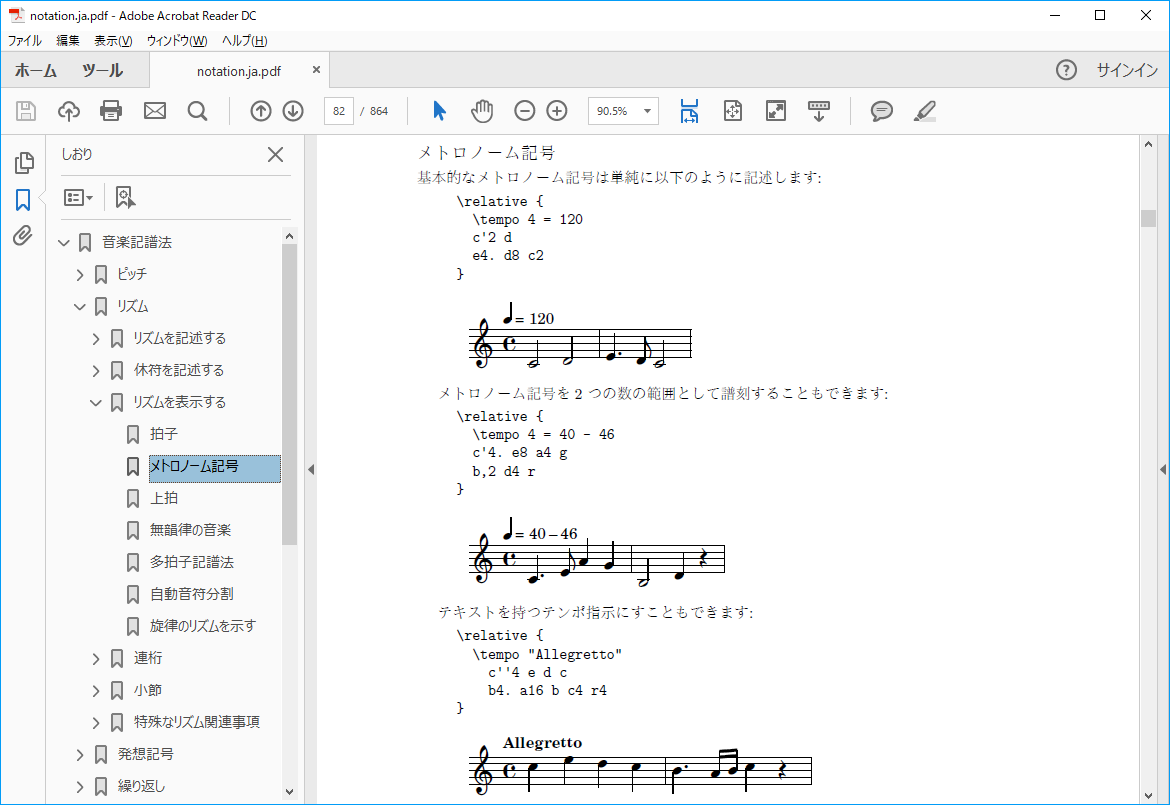
\includegraphics[width=0.95\linewidth]{notation-ja-capture.png}
  \caption{PDFの例(「しおり」が左に表示されている)}
  \label{fig:notation-ja-capture}
\end{figure}

\subsection{ハイパーリンク}

ハイパーリンクも便利な機能である。
PDFでリンクが設定されている場所をクリックすると、
設定された場所へジャンプすることができる。
リンク先としてはURLだけでなく、
同じPDF内のどこかや他のPDF内のどこかも指定できる。

また、PDF外部からリンクできるように、
名前付きアンカーとして機能するnamed destination
(本稿では宛先名と呼ぶ)を設定できる。
例えば、節に宛先名を設定しておくと、
PDF相互間でリンクする場合やHTMLからPDFへリンクする場合など
PDF外部(リモート)から節へジャンプするリンクを作ることができる。

LilyPondのマニュアルPDFは「学習マニュアル」や「記譜法リファレンス」など、
用途ごとに複数のPDFに分かれており、
Texinfoの機能でそれぞれのノード(節)に宛先名が設定され、
PDF間相互にリンクが張られている。
本稿PDFもhyperrefパッケージによりURLにリンクを指定してあるほか、
参考文献の引用番号や図表の参照番号から参照先へジャンプできるようにしている。
また、節はもちろん、図表や参考文献などにも宛先名が設定されており、
リモートからこうした場所を指定したリンクを作ることができる。

\subsection{フォント}

PDFにはドキュメントで使用しているフォントを埋め込むことができる。
これにより、PDF作成者が指定したフォントが存在しない環境でも、
PDF作成者の環境と同様の表示ができる。
この時、特に日本語を含むCJKフォントはグリフ数が多いため、
フォントを丸々フルセットで埋め込んでしまうとPDFファイルサイズが
大きくなってしまう。
そこで通常はPDF内で使用しているグリフのみを抜き出して埋め込む、
サブセット埋め込みをすることが多い。

また、逆にフォントを埋め込まずファイルサイズを小さくすることもできる。
この場合、PDF作成者が指定したフォントの情報をもとに、
PDFビュアーが環境中のフォントから同一のフォント、
もしくは同じような表示が望める代替フォントを探し出して使うことになる。
ファイルサイズは小さくできるが、
必ずしもPDF作成者の環境と同様の表示とならないことがあるので、
基本的にはフォントを埋め込む方法がとられる。

\section{LilyPond}

LilyPond \cite{lilypond}はソースファイル(テキストファイル)
をコンパイルすることで、
楽譜のPDFなどを生成することができる楽譜作成プログラムである。
ソースファイルの例を以下に示す。

\begin{center}
\tcbox[left=0mm,right=0mm,top=0mm,bottom=0mm]%
      {\lstinputlisting[linewidth=0.9\linewidth]{la_primavera-core.ly}}
\end{center}

このソースから生成した楽譜を図\ref{fig:la_primavera}に示す。
この図は実際にLilyPondで生成したPDFを\hologo{LuaLaTeX}の原稿に
貼り付けたものである。
その他に図\ref{fig:invention1}, \ref{fig:fur_elise}にも楽譜の例を示している。
これらによって、本稿のPDFそのものが複数の図を貼り付けたPDFとなり、
Extract PDFmarkによるファイルサイズ削減の
サンプルとなっている。

\begin{figure}
  \centering
  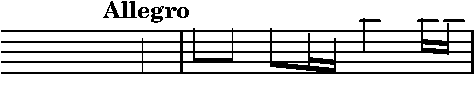
\includegraphics[scale=0.8]{la_primavera.pdf}
  \caption{楽譜の断片(ヴィヴァルディ「春」より)}
  \label{fig:la_primavera}
\end{figure}

\section{Texinfo}

Texinfo \cite{texinfo}はGNU公式文書フォーマットであり、
楽譜作成プログラムLilyPondを含め
GNU関連プロジェクトのドキュメント形式として広く使われている。
Texinfo形式で書かれたファイルを1つ用意すれば
HTMLやPDFをはじめとする様々な形式のドキュメントを出力することができる。
HTMLなどを出力する際にはスクリプトなどで変換処理が行われるが、
PDFを出力する際には\TeX が使われる。
この際には\LaTeX ではなく\hologo{plainTeX}が使われるが、
図を張り付けたPDFを作成するワークフローは基本的に\LaTeX と同様のため、
本稿では基本的にTexinfoと各種\LaTeX を区別しないこととする。
以下に、Texinfo形式ファイル冒頭部分の抜粋を例として示す。

\begin{tcolorbox}[left=0mm,right=0mm,top=0mm,bottom=0mm]
\begin{lstlisting}
\input texinfo-ja.tex

@documentencoding UTF-8
@documentlanguage ja

@settitle 吾輩は猫である
@afourpaper

@titlepage

@title 吾輩は猫である
@author 夏目漱石

これは日本語Texinfoファイルのサンプルとし
...
\end{lstlisting}
\end{tcolorbox}

1行目でTexinfoのコマンド等を定義する\hologo{plainTeX}用マクロを読み込み、
2行目から\verb|@|で始まるコマンドを用いて
マークアップしていくようになっている。

\section{\TeX で図を貼り込む}

\subsection{図のフォント}

各種\TeX ~/ \LaTeX で図を使った(貼り付けた)PDFを作成するには、
何らかの方法で作成した図のファイルを\TeX のソースファイルで取り込む
(\LaTeX なら\verb|\includegraphics|を使う)ことになる。
この際、グラフなどの文字を含んだ図はPDFファイルとして用意することが
多くなっていると思われる。
通常、特に何も考慮せずに文字を含んだPDFを作成すると、
使用しているフォントのサブセットが埋め込まれたPDFが生成される。
サブセットを埋め込む方法は、
様々な環境で同一の表示ができつつファイルサイズを抑えることができるため、
このPDFが最終目的物であれば正しい選択だといえる。

この方法で図\ref{fig:la_primavera}のPDFを生成したときの
フォント情報をPoppler \cite{poppler}付属のpdf\textcompwordmark
fontsを利用して表示したものを
表\ref{tbl:la_primavera-subset}に示す。emb列sub列ともにyesになっているので、
フォントが埋め込まれておりサブセットであるということがわかる。
また、name列のフォント名にサブセットであることを示す接頭辞が付いている。

\begin{table*}
  \centering
  \tcbox[colback=white,sharp corners,boxrule=1pt,%
    left=0mm,right=0mm,top=0mm,bottom=0mm]{\lstinputlisting[%
      basicstyle=\footnotesize\ttfamily,%
      lineskip=-1ex,%
      linewidth=0.95\linewidth]%
    {la_primavera-subset.txt}}
  \caption{「春」PDFフォント情報(オプション無指定、サブセット埋め込み)}
  \label{tbl:la_primavera-subset}
\end{table*}

しかし、こうしたPDFを図として\TeX ソースファイルで大量に取り込んだ場合、
\TeX が出力するメインPDFには、
各々の図PDFに埋め込まれていたフォントがすべてそのまま埋め込まれてしまう。
複数の図で同じフォントが使われていることも多いと思われるが、
重複は解消されず、そのまま同じフォントが複数回埋め込まれてしまい、
ファイルサイズの増加につながってしまう。

\subsection{フォント重複の解消}

この問題を解消するには、図PDF作成時のフォント埋め込み方法を工夫し、
\TeX が出力したPDFをGhostscriptで処理して
フォントの埋め込みを制御する方法がある。
制御の方法としては大きく2つのアプローチがある。

\subsubsection{フルセット(非サブセット)埋め込み}

図PDFに埋め込まれているフォントを、サブセット埋め込みではない、非サブセット、
つまり全グリフをフルセットで埋め込むようにするアプローチである。
これによって図PDFのサイズは増え、
この図を張り付けた\TeX 出力PDFも非常に大きなサイズになってしまう。
しかし、このPDFでは、
同じフォントはすべてフルセットで埋め込まれた全く同じものになるので、
後から重複しているものを取り除いて統合することができる。
さらに、統合後に使われているグリフのみを含んだサブセット化をすれば、
必要なフォントの必要なグリフが1つだけ埋め込まれている状態にできる。
これにより、中間ファイルのサイズは大きくなってしまうものの、
最終ファイルの大きさを減らすことができる。

このアプローチは、
中間ファイルのサイズが大きくなるというデメリットがあるものの、
比較的フローが単純でわかりやすい。
しかし、うまくいっているように見えても問題を抱えていることがある。
まず、正しいフルセット埋め込みのPDFを作成することが困難である。
PDF生成エンジンとしてもよく使われるGhostscriptは
最新バージョンの9.22rc2でもフルセット埋め込みに問題がある。
表面的にはフルセット埋め込みができたように見えるが、
実際にはすべてのグリフを含んでいない「バグ」がある\cite{gs-non-subset}。

さらに、フォントを統合する方法が困難である。
従来、こういったフォントの統合およびサブセット化には
Ghostscriptが広く使われてきた。
Ghostscriptによるフォント統合は、バージョン9.16まではそのまま動作するが、
バージョン9.17から\verb|-dPDFDontUseFontObjectNum|オプションが
必要となった。
そして、このオプションはバージョン9.21までは動作するが、
9.22rc1で削除されてしまった\cite{gs-PDFDontUseFontObjectNum}。
gs-develメーリングリストでの議論によると、
そもそも重複するフォントを削除する動作は意図していたものではなく、
この動作により文字化けを起こすことがあるので廃止した、
というような説明が読める\footnote{議論の中で、
MuPDFなら重複フォント削除ができるという情報もあったが、
そもそも正しいフルセット埋め込みPDFが用意できないので
試すことができない。}。

また、フォント統合を目的の一つとしている
pdfsizeopt \cite{pdfsizeopt}というツールがあるが、
グリフ数256を超えるフォントの処理に未対応である\cite{pdfsizeopt14}。
和文フォントはもちろんグリフ数256を超えるし、
欧文フォントもギリシャ文字やキリル文字のグリフを
含んでいるなどグリフ数が256を超えるフォントが多く、
実質的に使用できない。

そして、何らかの方法でフォントの統合ができたら
サブセット化する。
これにはGhostscriptを使うことができる。
いずれにせよ、フルセット埋め込みによるアプローチは、
表面的には正常に動作したように見えても、
どこかで何らかの文字化けや、その他の問題が発生している可能性があるので
注意しなければならない。

\subsubsection{非埋め込み}

図PDFをフォント非埋め込みにするアプローチである。
これにより、その図を貼り付けた\TeX 出力PDFも、
図で使われているフォントについて非埋め込みとなる。
もちろんこのままでは表示環境によって異なる表示となってしまう。
例えばLilyPondの場合、音符もフォントで表現しており、
通常の環境には音符フォントはインストールされておらず、
代替できるようなフォントもないため、音符の表示ができなくなってしまう。
そこで、\TeX 出力PDFへ必要なフォントを埋め込む処理を行う。
このアプローチは中間ファイルのサイズが小さいままでフローを進めることができ、
大量の図を貼り付けたドキュメントであってもディスク容量の消費量を抑制できる。

この方法で図\ref{fig:la_primavera}のPDFを生成したときの
フォント情報を表\ref{tbl:la_primavera}に示す。
emb列sub列ともにnoになっているので、
フォントが埋め込まれていないことがわかる。name列に接頭辞もついていない。
Emmentaler-20フォント(音符フォント)が3回登場するが、
これは後でフォントを統合するため3種類の異なるエンコーディングを
定義して使用しているからである\footnote{こうしないと
楽譜の断片毎に都度生成された異なったエンコーディングが使われ、
後で統合できなくなることがある。}。

\begin{table*}
  \centering
  \tcbox[colback=white,sharp corners,boxrule=1pt,%
    left=0mm,right=0mm,top=0mm,bottom=0mm]{\lstinputlisting[%
      basicstyle=\footnotesize\ttfamily,%
      lineskip=-1ex,%
      linewidth=0.98\linewidth]%
    {la_primavera.txt}}
  \caption{「春」PDFフォント情報(非埋め込み)}
  \label{tbl:la_primavera}
\end{table*}

埋め込み処理にはGhostscriptを使うことができるが、
使用するフォントそのものを何らかの方法でGhostscriptへ渡す必要がある。
基本的には、特定のディレクトリへフォントファイルを置いたり、
Ghostscriptの設定ファイルを編集したりする必要があるなど、
非常に煩雑であり、ドキュメント生成を自動化することも困難である。
また、GhostscriptはOTCフォント\footnote{OpenType/CFF Collectionフォント}を
直接ロードすることができないため、そのままではOTCフォントが使えない
という問題もある。

一方、Ghostscriptはフォントが埋め込まれたファイルを読み込むことができるので、
これを利用してフォントを渡す方法がある。
フォントが埋め込まれたPostScriptファイルと同じ形式で、
フォントリソースのみが書かれているファイルを一時的に用意し、
PDF処理時にPDFとともにGhostscriptへ入力ファイルとして渡す方法である。
この方法であればOTCフォントも中身のCFFを抽出して、
フォントリソースとして書き出すことによって利用可能である。
特定のディレクトリへファイルを配置する必要もなく、
設定ファイル編集も不要なので自動化にも都合が良い。
LilyPondには、このためにフォントリソースを別途出力する
オプション\verb|-dfont-export-dir|があり、
マニュアルPDFはこの方法を採用し、\verb|make doc|で自動的に生成される。
また、本稿PDFもこの方法を使っている。

いずれにしても、Ghostscriptへフォントを渡さなければならないので、
フルセット埋め込みのアプローチと比較すると複雑であることは否めない。
また、非埋め込みのアプローチでは、
図を作成したときのフォントの種類やエンコーディングなどによって、
最終的に出力したPDFで文字化けやその他の問題が発生する可能性があるので、
注意が必要であることには変わりはない。

\subsection{Ghostscriptで失われるもの}

いずれのアプローチであっても
Ghostscriptは重要な役割を果たしている。
具体的には\TeX 出力PDFをGhostscriptで処理する、
というフローを経る必要がある。
しかし、Ghostscriptは元々のPDFに存在した情報のうち、
いくつかを保持することができず失ってしまう。

一つはページモードの情報である。
例えばhyperrefパッケージで「しおり」を作成し、
PDFを開いたときに「しおり」が開かれた状態になるよう設定したとしても、
そのPDFをGhostscriptで処理すると
「しおり」が開かれない状態に変わってしまう
\footnote{「しおり」の内容は保持される。}。
もっと深刻なのは、宛先名の情報である。
どこかのPDFドキュメントから別のPDFドキュメントの特定の項目へ
ジャンプするリンクを貼ったとしても、
Ghostscriptで処理をすると飛び先が意図した項目の場所ではなく、
ドキュメントの先頭ページになってしまう。
PDF相互間のリンクでなくても、宛先名をアンカーとして指定したURLが
常にドキュメントの先頭を開くようになってしまうようになる。

\section{Extract PDFmark}

Ghostscript処理で失われる情報を保持するため
Extract PDFmark \cite{extractpdfmark}を利用できる。

\subsection{インストール}

Extract PDFmarkはDebian 9 stretchやUbuntu 17.04 Zesty Zapusで
extractpdfmarkパッケージとなっており、
その他Linuxディストリビューションでもパッケージ化されているものがある。
また、Cygwinでもパッケージになっている。
こうした環境ではパッケージを使って簡単にインストールできる。
その他の環境ではソースからインストールする必要があるが、
Autotoolsで作成されているので比較的簡単にできると思う。

\subsection{仕組み}

Extract PDFmarkの仕組みを述べる。

\subsubsection{pdfmark}

pdfmark \cite{pdfmark}は、PDFの機能をPostScriptの中に
記述するためのものである。
例えば、PDFを開いた際に「しおり」が開かれるようにするページモード設定は、
以下のようになる。

\begin{tcolorbox}[left=0mm,right=0mm,top=0mm,bottom=0mm]
\begin{lstlisting}
[ /PageMode /UseOutlines /DOCVIEW pdfmark
\end{lstlisting}
\end{tcolorbox}

このようなpdfmarkを含んだPostScriptファイルをGhostscriptでPDFへ変換すると、
生成されたPDFは開いた際に「しおり」が開かれるようになる。
同様に宛先名についてもpdfmarkで設定できる。

\subsubsection{抽出}

PDFの仕様は公開されているので、
\TeX 出力PDFからページモードの情報や宛先名の情報を読み取ることが可能である。
Extract PDFmarkはPoppler \cite{poppler}ライブラリを使ってこれらを読み取って
pdfmarkの形式で出力するものである。
コマンドライン引数に対象となるPDFファイルを指定すると
標準出力へpdfmarkを出力する。

\subsubsection{Ghostscriptの入力}

Ghostscriptは一度に複数の入力を取り扱うことができ、
入力ファイルごとに形式がPostScriptなのかPDFなのか個別に判断する。
そこで、pdfmarkのみ記述されたPostScriptファイルと
PDFファイルをともに与えることで、
入力になっているPDFに設定されている機能とは関係なく、
もう一つの入力であるpdfmarkの機能が適用されたPDFを出力することができる。

これを利用することにより、
ページモードや宛先名が失われるGhostscriptであっても、
これらを保持したまま処理をすることができるようになる。
具体的には、まず、Ghostscript処理前の\TeX 出力PDFから、
Extract PDFmarkを利用してページモードと宛先名をpdfmark形式で抽出する。
次に、Ghostscript処理へ抽出したpdfmarkと\TeX 出力PDFを一緒にかける。
そうすると、\TeX 出力PDFで指定されていたページモードと宛先名が、
そのまま保持された状態でGhostscript処理されたPDFを得ることができる。

\subsection{使い方}

フォント非埋め込みのアプローチで、
フォントリソースのみが含まれているPostScriptファイルを
\verb|fonts/*.font.ps|へ置いたとすると、以下のような使い方となる。

\begin{tcolorbox}[left=0mm,right=0mm,top=0mm,bottom=0mm]
\begin{lstlisting}[basicstyle=\footnotesize\ttfamily]
$ extractpdfmark TeX出力.pdf > 抽出pdfmark.ps
$ gs -q -dBATCH -dNOPAUSE -sDEVICE=pdfwrite \
    -sOutputFile=最終.pdf \
    fonts/*.font.ps \
    TeX出力.pdf 抽出pdfmark.ps
\end{lstlisting}
\end{tcolorbox}

\subsection{注意事項}

Ghostscript 9.19までは、
一部の宛先名を正しく扱うことができない\cite{gs-919-bug}ため、
英数字以外の名前を扱うにはGhostscript 9.20以降が必要となる。
Texinfoはノード名がそのまま宛先名になるので、
この制限に触れてしまう可能性が高い。

非埋め込みの図PDFを使うアプローチで、
LilyPondが生成する図PDFにTrueTypeフォントを使うと
文字化けを起こすことがある。
欧文フォントではWinAnsiエンコーディング範囲外のグリフ
(例えばギリシャ文字など)が文字化けするし、
和文フォントでは全体が文字化けする。
そのため、LilyPondではフォント非埋め込みPDFを出力する
オプション\verb|-dgs-neverembed-fonts|が指定されても、
あえてTrueTypeフォントは埋め込むようにしている。

\section{おわりに}

\begin{figure*}
  \centering
  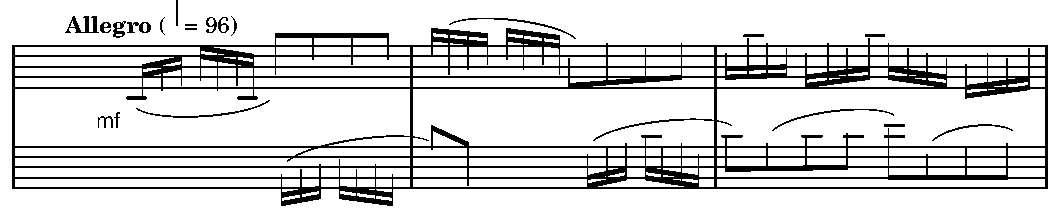
\includegraphics[scale=0.8]{invention1.pdf}
  \caption{楽譜の断片(「インヴェンション第一番」より)}
  \label{fig:invention1}
\end{figure*}

本稿ではExtract PDFmarkによって、
ファイルサイズの小さいPDFを得る方法を説明した。
\TeX などで同じフォントが埋め込まれた多数の図PDFを貼り込むと、
結果として生成されるPDFには同じフォントが重複して埋め込まれ、
ファイルサイズの増加につながる。
Ghostscript処理により埋め込み制御ができるが、
PDFの開き方やリモートからのリンクが失われる。
Extract PDFmarkにより、
これらを失わずにファイルサイズの小さいPDFを得ることができる。

LilyPondのマニュアルPDFは、2016年11月リリースのバージョン2.19.51まで
サブセット埋め込みの図PDFを使用していたが、
翌月リリースの2.19.52からExtract PDFmarkを採用し
非埋め込みの図PDFを使用している。
これによりPDF生成に要するディスク容量は4.6 GBから3.4 GBへ減少、
マニュアルPDFの合計サイズも280 MBから104 MBと半減以下にすることができた。
英語版の記譜法マニュアル(notation.pdf)のサイズは36 MBから9.9 MBと
1/3以下になっている\cite{issue5000}。

なお、各ツールのオプションや動作は本稿執筆時点のものである。
特にLilyPondは最新バージョン2.19.65を用いたが、
Ghostscript 9.22rc1の\verb|-dPDFDontUseFontObjectNum|廃止に
端を発する議論を受け、
次期2.20に向けオプションや一連の動作を見直している最中であり、
今後変更される予定である。
もともと、フォント重複によるファイルサイズ増を抑える方法としては、
フルセット埋め込みによるアプローチの方が有名で有力だと考えていたが、
本稿執筆中の2017年9月にこのような大きな動きがあり、
まさにひっくり返ってしまった感が強い。
一方で議論を通じて様々な知見が得られ大変勉強になったし、
本稿に最新の有用な情報を盛り込むことができたと考えている。
この議論はgs-develメーリングリストやlilypond-develメーリングリスト
のアーカイブで読むことができる\cite{gs-devel}\cite{lilypond-devel}。

最後に、本稿関連ファイルを文献\cite{tr-texconf2017}で公開している。
ソースファイルや最終PDFだけでなく、
図PDFなど中間ファイルも用意しているので、
参考にしていただけると幸いである。

\begin{flushright}
(2017年9月30日提出)
\end{flushright}

\begin{figure}
  \centering
  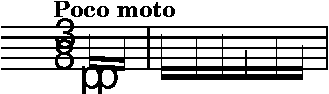
\includegraphics[scale=0.8]{fur_elise.pdf}
  \caption{楽譜の断片(「エリーゼのために」より)}
  \label{fig:fur_elise}
\end{figure}

\begin{thebibliography}{99}

\bibitem{extractpdfmark} Extract PDFmark. \\
  \url{https://github.com/trueroad/extractpdfmark}. \\
  \url{http://www.ctan.org/pkg/extractpdfmark}.

\bibitem{lilypond} 楽譜作成プログラムLilyPond. \\
  \url{http://lilypond.org}.

\bibitem{texinfo} GNU公式文書フォーマットTexinfo. \\
  \url{https://www.gnu.org/software/texinfo/}.

\bibitem{poppler} Poppler. \\
  \url{https://poppler.freedesktop.org/}.

\bibitem{gs-non-subset} gs-develメーリングリスト2017年9月より. \\
  \url{https://ghostscript.com/pipermail/gs-devel/2017-September/010015.html}.

\bibitem{gs-PDFDontUseFontObjectNum} gs-develメーリングリスト2017年9月より. \\
  \url{https://ghostscript.com/pipermail/gs-devel/2017-September/009988.html}.

\bibitem{pdfsizeopt} pdfsizeopt. \\
  \url{https://github.com/pts/pdfsizeopt}.

\bibitem{pdfsizeopt14} Type1CConverter and Type1CGenerator
  with fonts with more than 256 glyphs. \\
  \url{https://github.com/pts/pdfsizeopt/issues/14}.

\bibitem{pdfmark} pdfmark Reference. \\
  \url{http://kb2.adobe.com/jp/cps/511/511364.html}. \\
  \url{http://www.adobe.com/content/dam/Adobe/en/devnet/acrobat/pdfs/pdfmark_reference.pdf}.

\bibitem{gs-919-bug} Ghostscript bug 696974. \\
  \url{https://bugs.ghostscript.com/show_bug.cgi?id=696974}.

\bibitem{issue5000} Issue 5000:
  Add using Extract PDFmark for document building. \\
  \url{https://sourceforge.net/p/testlilyissues/issues/5000/}.

\bibitem{gs-devel} gs-develメーリングリスト2017年9月アーカイブ. \\
  \url{https://ghostscript.com/pipermail/gs-devel/2017-September/date.html}.
\bibitem{lilypond-devel} lilypond-develメーリングリスト2017年9月アーカイブ. \\
  \url{http://lists.gnu.org/archive/html/lilypond-devel/2017-09/index.html}.

\bibitem{tr-texconf2017} TeXConf 2017 files. \\
  \url{https://github.com/trueroad/tr-TeXConf2017}.

\end{thebibliography}

\end{document}
